\documentclass{report}

\usepackage[T1]{fontenc}
\usepackage[utf8]{inputenc}
\usepackage[brazilian]{babel}
\usepackage{graphicx}
\usepackage[export]{adjustbox}[2011/08/13]
\usepackage{float}
\usepackage[pdftex]{hyperref}
\usepackage{epstopdf}
\usepackage{etoolbox}
\usepackage{amsmath}
\usepackage{amsfonts}
\usepackage{amssymb}
\usepackage{caption}
\usepackage{subcaption}
\usepackage{setspace}
\usepackage{tikz}
\usepackage{listings}
\usepackage{xcolor} 

\bibliographystyle{apalike}
\patchcmd{\thebibliography}{\section*}{\section}{}{}
\newcommand{\R}{\ensuremath{\mathbb{R}}}
\newcommand{\Prob}{\ensuremath{\mathbb{P}}}
\newcommand{\K}{\ensuremath{\mathbb{K}}}
\newcommand{\U}{\ensuremath{\mathbb{U}}}
\newcommand{\N}{\ensuremath{\mathbb{N}}}
\newcommand{\Lg}{\ensuremath{\mathbb{L}}}
\newcommand{\T}{\ensuremath{\rm Tr}}
\newcommand{\sg}{{\sigma(x_k)}}

\newcommand{\G}{\ensuremath{\mathcal{G}}}
\newcommand{\F}{\ensuremath{\mathcal{F}}}
\newcommand{\C}{\ensuremath{\mathcal{C}}}
\newcommand{\E}{\ensuremath{\mathcal{E}}}
\newcommand{\Hn}{\ensuremath{\mathcal{H}}}
\newcommand{\Hoo}{\ensuremath{\mathcal{H}_\infty}}
\newcommand{\Hop}{\ensuremath{\mathcal{H}_{op}}}
% --------------------------------------------------
\newtheorem{theo}{Teorema}
\newtheorem{exa}{Exemplo}
\newtheorem{lemm}{Lema}
\newtheorem{coro}{Corolário}
\newtheorem{defn}{Definição}[section]

\begin{document}
\input{capa.tex}

\onehalfspacing
\section{Objetivos}

\section{Retificador monofásico}
\begin{figure}[H]
	\centering
	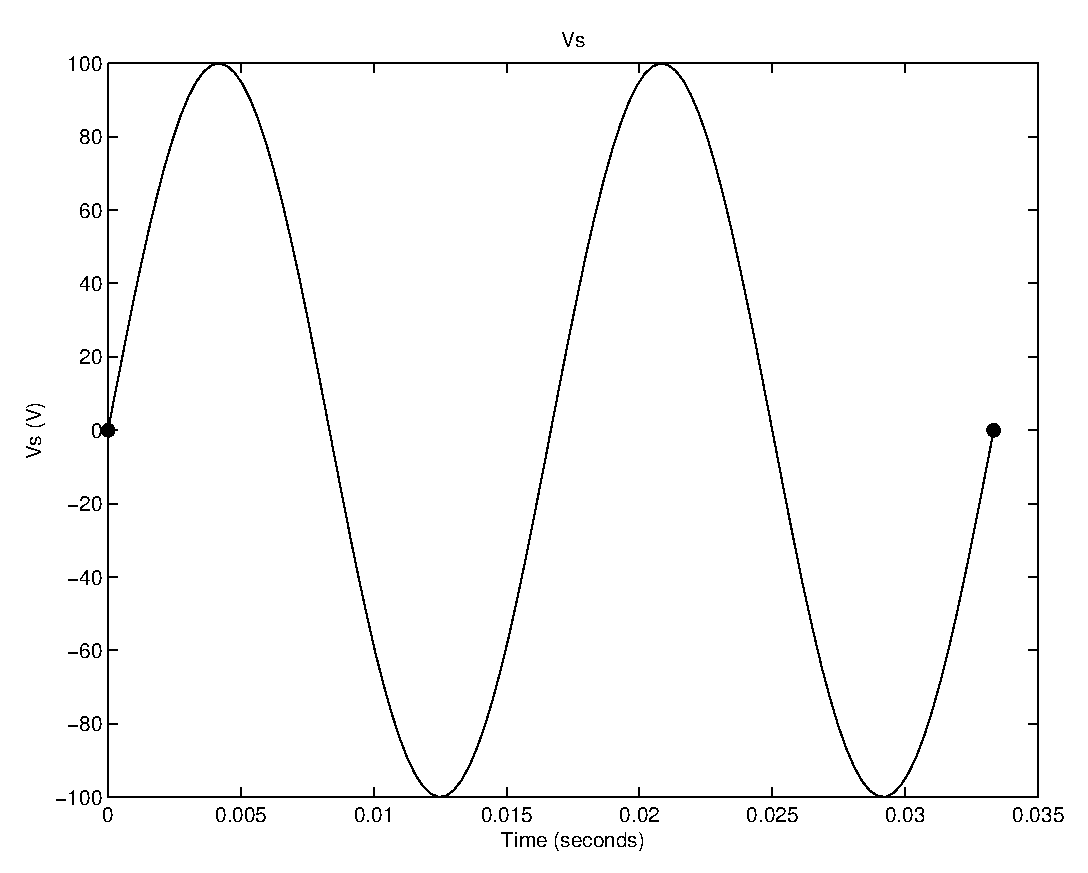
\includegraphics[width=0.7\linewidth]{matlab/mono_vs}
	\caption{Tensão da fonte para retificador monofásico}
	\label{fig:mvs}
\end{figure}
\begin{figure}[H]
	\centering
	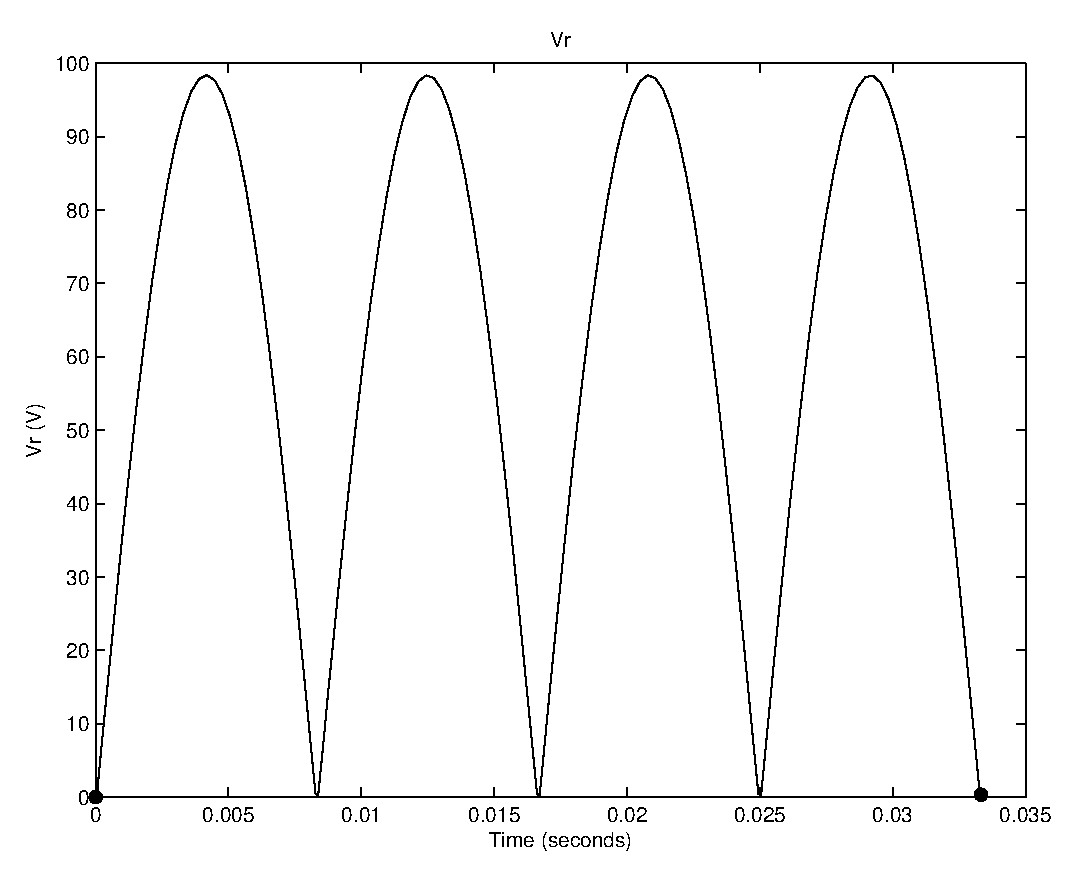
\includegraphics[width=0.7\linewidth]{matlab/mono_vr}
	\caption{Tensão na carga para retificador monofásico}
	\label{fig:mvr}
\end{figure}
\begin{figure}[H]
	\centering
	\includegraphics[width=0.7\linewidth]{matlab/mono_ir}
	\caption{Corrente na carga para retificador monofásico}
	\label{fig:mir}
\end{figure}

\foreach \n in {1,...,4}{
	\begin{figure}[H]
		\centering
		\includegraphics[width=0.7\linewidth]{matlab/mono_d\n i}
		\caption{Corrente no diodo \n  para retificador monofásico}
		\label{fig:md\n i}
	\end{figure}
	
	\begin{figure}[H]
		\centering
		\includegraphics[width=0.7\linewidth]{matlab/mono_d\n v}
		\caption{Tensão no diodo \n  para retificador monofásico}
		\label{fig:md\n v}
	\end{figure}
}

\section{Retificador trifásico}
\begin{figure}[H]
	\centering
	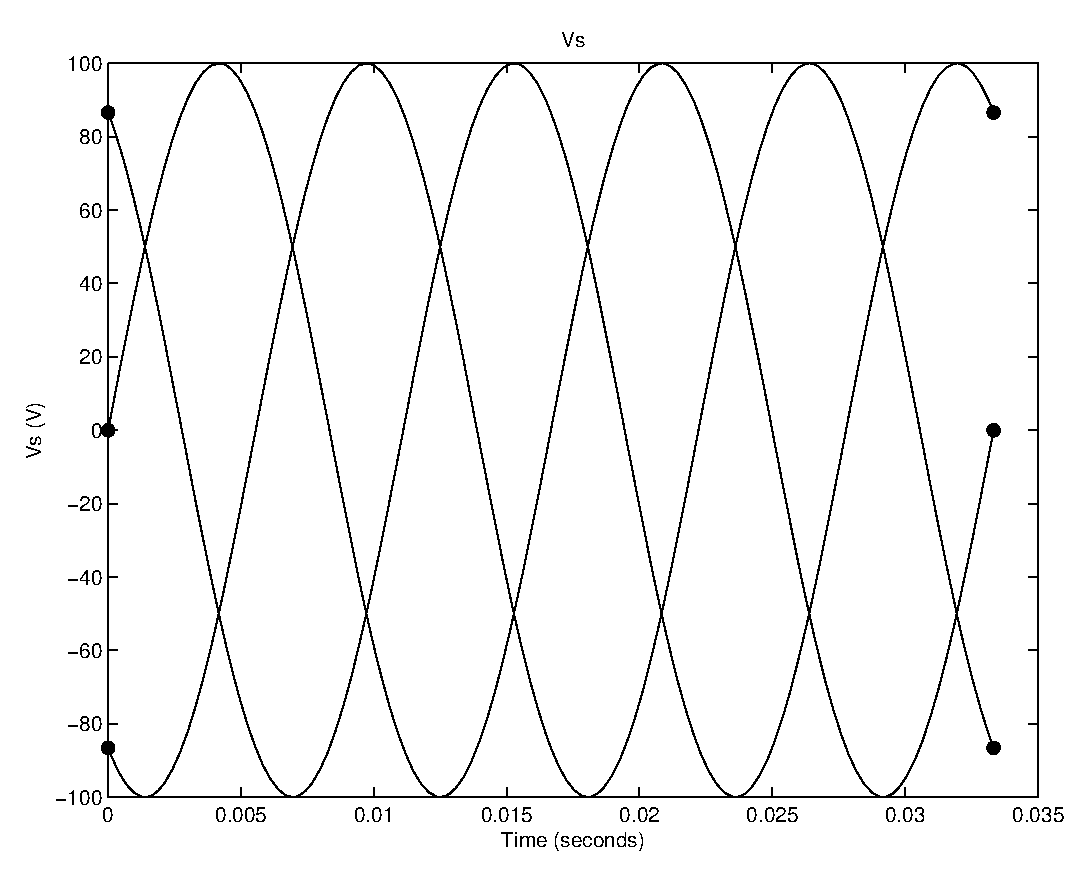
\includegraphics[width=0.7\linewidth]{matlab/tri_vs}
	\caption{Tensões das fontes para retificador trifásico}
	\label{fig:tvs}
\end{figure}
\begin{figure}[H]
	\centering
	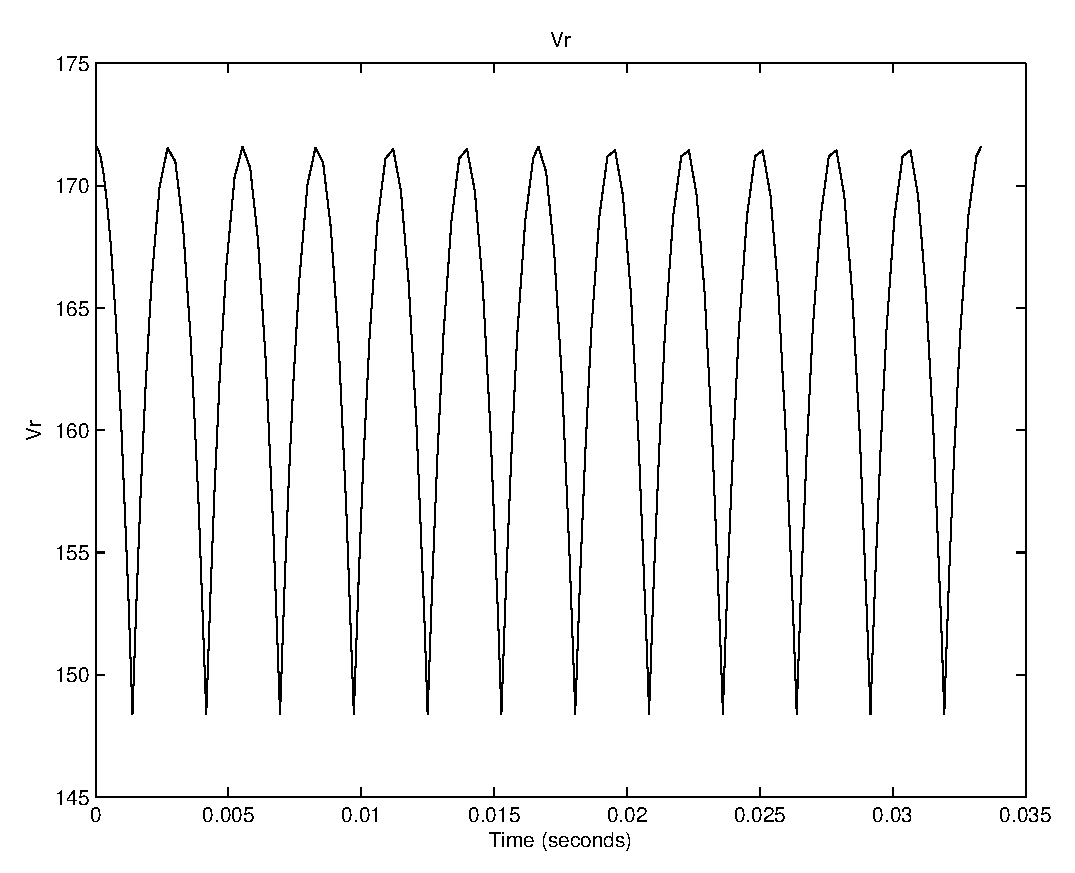
\includegraphics[width=0.7\linewidth]{matlab/tri_vr}
	\caption{Tensão na carga para retificador trifásico}
	\label{fig:tvr}
\end{figure}
\begin{figure}[H]
	\centering
	\includegraphics[width=0.7\linewidth]{matlab/tri_ir}
	\caption{Corrente na carga para retificador trifásico}
	\label{fig:tir}
\end{figure}

\foreach \n in {1,...,6}{
	\begin{figure}[H]
		\centering
		\includegraphics[width=0.7\linewidth]{matlab/tri_d\n i}
		\caption{Corrente no diodo \n  para retificador trifásico}
		\label{fig:td\n i}
	\end{figure}
	
	\begin{figure}[H]
		\centering
		\includegraphics[width=0.7\linewidth]{matlab/tri_d\n v}
		\caption{Tensão no diodo \n  para retificador trifásico}
		\label{fig:td\n v}
	\end{figure}
}

\bibliography{mybib.bib}
\end{document}

